\documentclass[11pt]{article}
\usepackage[margin=1in]{geometry}
\usepackage{amsmath,amssymb,booktabs,microtype,graphicx}
\usepackage[hidelinks]{hyperref}

\title{Scoring accuracy in \texttt{llp\_forward}\\
\large A distance-based metric, and the 2026-08 campaign expressed in it}
\author{HEPBench}
\date{2026-08-08}

\newcommand{\Nsig}{N_{\mathrm{sig}}}
\newcommand{\mphi}{m_\phi}

\begin{document}
\maketitle

\begin{abstract}
\noindent
This note defines how \texttt{llp\_forward} measures the accuracy of an agent's
answer, and reports the 2026-08 campaign in those terms. The proposal is: report
the \emph{distance} $D$, the median $|\log_{10}|$ ratio between the agent's
observable and the reference's, in decades; score it as $10^{-D}$, which is
exactly the reciprocal of the factor the agent is off by and contains no free
parameter; and keep the statistical significance $z=D/\sigma$ as a separate
\emph{test} of whether a discrepancy is real, never as a score. The two reach
contour edges are reported separately, because they measure different physics
and, on this campaign, differ by up to a factor 19 within a single trial.
\end{abstract}

\section{Scope}

The task asks an agent to compute the sensitivity of a forward long-lived
particle search to a muon-philic scalar $\phi$. What is graded is what it
computes, not how: a signal yield $\Nsig(\mathrm{search},\mphi,g)$ on a declared
set of points, and the reach contour that follows from it. This note covers only
the \emph{accuracy} stages. Completion gates (did the required files appear) and
the symbolic width check are unaffected and are not discussed.

Section~\ref{sec:obs} defines the observables, \S\ref{sec:D} the distance,
\S\ref{sec:score} the score, \S\ref{sec:z} the significance test, and
\S\ref{sec:report} what a results table must contain. \S\ref{sec:campaign}
applies all of it to the 2026-08 campaign. \S\ref{sec:rejected} records what was
tried and rejected, and why, so it is not re-proposed.

\section{The observables}\label{sec:obs}

Three observables are graded, and they are kept \textbf{separate}.

\paragraph{Yield.} The reference declares $n=48$ points
$(\mathrm{search}_i,\, m_{\phi,i},\, g_i)$ --- four couplings at each of twelve masses,
placed to bracket the sensitive region --- each with a reference value
$N^{\mathrm{ref}}_{\mathrm{sig},i}$. The agent's own scan is interpolated linearly in
$(\log_{10} g,\ \log_{10}\Nsig)$ onto those same couplings, giving
$N^{\mathrm{agent}}_{\mathrm{sig},i}$. Both sides are therefore evaluated at identical
$(\mathrm{search},\mphi,g)$, and no grid choice enters.

\paragraph{Reach contour, lower edge.} For each mass the reference reports the
band $[g_{\mathrm{lo}},g_{\mathrm{hi}}]$ within which $\Nsig\ge3$. The grader
reconstructs the same crossings from the agent's scan. The lower edge is
\emph{production-limited}: below it the coupling is too weak, too few $\phi$ are
made, and those that are live long enough to fly through the volume undecayed.

\paragraph{Reach contour, upper edge.} The same construction at the other
crossing. This edge is \emph{lifetime-limited}: above it $c\tau\propto g^{-2}$ is
so short that the $\phi$ decays before reaching the volume.

\medskip
\noindent
\textbf{The two edges are never pooled.} They are set by different physics, they
respond differently to methodology, and on the 2026-08 campaign a single trial
can sit at $0.0028$ dex on the lower edge and $0.066$ on the upper --- a factor
$19$. Averaging them turns a bimodal distribution into a misleading unimodal one
and destroys the campaign's most informative result (\S\ref{sec:campaign}).

\section{The distance $D$}\label{sec:D}

For each graded point $i$ define the signed residual in decades,
\begin{equation}
  d_i \;=\; \log_{10}\!\left(\frac{X^{\mathrm{agent}}_i}{X^{\mathrm{ref}}_i}\right),
\end{equation}
where $X$ is $\Nsig$ for the yield observable and the edge coupling
$g_{\mathrm{lo}}$ or $g_{\mathrm{hi}}$ for the contour observables. The distance
for one trial is the median of the magnitudes,
\begin{equation}
  D \;=\; \operatorname{median}_i\,|d_i| \qquad [\text{decades, ``dex''}].
\end{equation}
A cell's $D$ is the median over its trials of the per-trial $D$.

\paragraph{Why the logarithm.} The observable spans roughly eight decades across
the graded points. Only a ratio is meaningful, and $\log_{10}$ makes the ratio
additive and symmetric: being high by $2\times$ and low by $2\times$ both give
$d=\pm0.301$.

\paragraph{Why the median.} The residual distribution has genuine outliers ---
points where an agent produced nothing sensible --- and a mean would be
dominated by them. The median reports the typical point. Its spread is reported
separately rather than being folded in (\S\ref{sec:report}).

\paragraph{Coverage.} A point contributes only if the agent's scan spans the
required coupling. \emph{Coverage} is the fraction of graded points that
contributed. Rows at coverage $<1$ are not comparable to rows at $1$, since $D$
was computed on a subset.

\paragraph{Stability.} $D$ is a property of the agent, not of the reference's
current precision. When the reference was rebuilt on 2026-08-07 --- the parent
decay-length sampling corrected and the parent flux regenerated at ten times the
statistics, improving its own $\sigma$ by a factor $17$ --- every cell's $D$
moved by at most $0.04$ dex and the ordering did not change. A metric that
survives that is measuring the thing it claims to measure.

\section{The score}\label{sec:score}

\begin{equation}
  \boxed{\;\text{score} \;=\; 10^{-D}\;}
\end{equation}

Because $D$ is a median of $|\log_{10}|$ ratios, $10^{-D}$ is exactly
\emph{the reciprocal of the median factor by which the agent is wrong}. The
anchors are not chosen; they follow:

\begin{center}
\begin{tabular}{lcc}
\toprule
agent is off by & $D$ & score \\ \midrule
nothing            & $0$     & $1.000$ \\
$25\%$             & $0.097$ & $0.800$ \\
a factor $2$       & $0.301$ & $0.500$ \\
a factor $10$      & $1$     & $0.100$ \\
a factor $100$     & $2$     & $0.010$ \\
\bottomrule
\end{tabular}
\end{center}

\noindent This is the central proposal, and its properties are the argument for
it:

\begin{enumerate}
\item \textbf{No free parameter.} There is no tolerance, no width, no
  $\sigma$ in the score. The only choice is the base of the logarithm, and that
  is already fixed by the unit $D$ is quoted in. There is nothing for a reader
  to object to as arbitrary.
\item \textbf{Directly interpretable.} A score of $0.5$ means ``typically off by
  a factor of two.'' No calibration table is needed to read the number.
\item \textbf{Bounded and monotone.} $10^{-D}\in(0,1]$, strictly decreasing in
  $D$, saturating at neither end. Better agents are always separated.
\item \textbf{Aggregation-invariant.} Since $x\mapsto10^{-x}$ is strictly
  monotone, quantiles commute with it:
  $\operatorname{median}_i(10^{-|d_i|}) = 10^{-\operatorname{median}_i|d_i|}$.
  Scoring each point and then aggregating gives the same answer as aggregating
  and then scoring, so the reported $D$ and the reported score cannot disagree.
\item \textbf{Invariant to reference improvements.} It inherits the stability of
  $D$. Sharpening the reference does not silently rescale published scores.
\end{enumerate}

Figure~\ref{fig:score} shows the function with the campaign placed on it.

\begin{figure}[htbp]\centering
  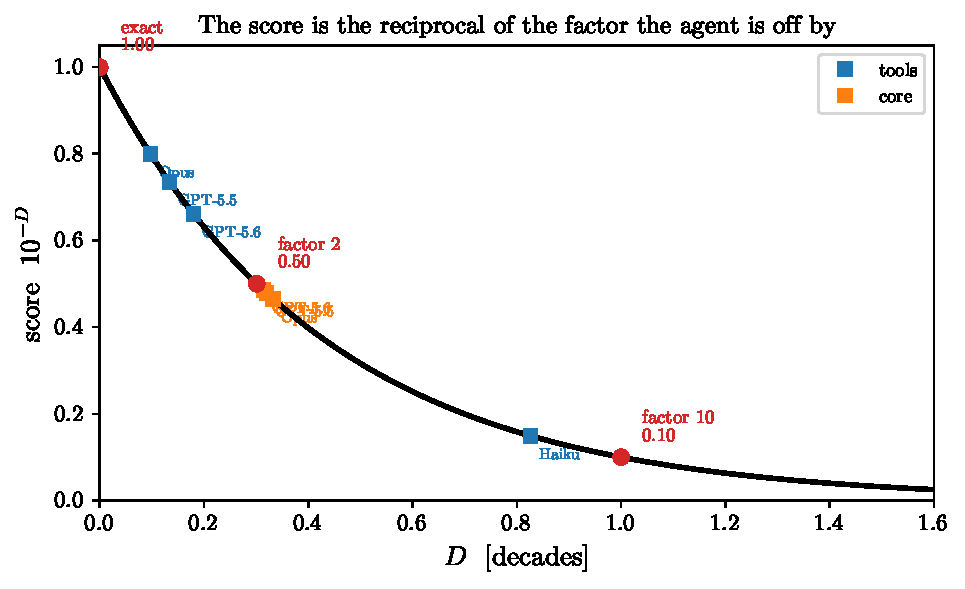
\includegraphics[width=0.78\textwidth]{figures/score_function.pdf}
  \caption{The score $10^{-D}$. Red markers are the parameter-free anchors; squares
  are the 2026-08 campaign cells on the yield observable.}
  \label{fig:score}
\end{figure}

\paragraph{Tail behaviour.} $10^{-D}$ never reaches zero: an agent wrong by
$100\times$ still scores $0.01$. If a hard pass/fail is wanted it should be
stated on $D$ directly --- ``within a factor of two'' is $D\le0.301$ --- which
is a physics statement rather than a tuned constant.

\section{Significance, as a test and not a score}\label{sec:z}

\subsection{The measured floor}

Two independent noise sources are known, both \emph{measured}:

\begin{itemize}
\item \textbf{The reference.} Two complete reference builds are made from
  independent $2\times10^6$-event Pythia fluxes (seeds 1000 and 2000) through
  one pipeline. For same-size independent samples the pair difference is
  $\sqrt2\,\sigma$, giving
  $\sigma_{\mathrm{ref}}^{\mathrm{yield}}=0.00188$ dex and
  $\sigma_{\mathrm{ref}}^{\mathrm{contour}}=0.00214$ dex.
\item \textbf{The agent.} Each tooled trial records its own Monte-Carlo sample
  sizes, and those records are accepted only after being checked against the
  trial's graded scan. The median statistical precision is
  $\sigma_{\mathrm{agent}}=0.00164$ dex.
\end{itemize}

Combining, and noting that near the lower edge $\Nsig\propto g^2$ so an edge
inherits half the yield error in dex,
\begin{equation}
  \sigma^{\mathrm{yield}} = 0.00249~\text{dex},\qquad
  \sigma^{\mathrm{contour}} = 0.00229~\text{dex},\qquad
  z \;=\; D/\sigma .
\end{equation}
Nothing here is chosen; every term is measured.

\subsection{What $z$ is for}

$z$ answers one question: \emph{is this discrepancy real, or could it be
sampling noise?} It is a hypothesis test, and it is used as one.

It cannot be a score. On this campaign $z$ ranges from $1.2$ to $1080$, and
mapping that to credit through $\exp(-z^2/2)$ gives every cell exactly $0.000$
--- correctly, because the errors are \emph{systematic}, not fluctuations.
Properly computed error bars make a systematic error look \emph{more}
significant, not less. Quoting ``$39\sigma$'' would also imply a $p$-value near
$10^{-330}$, which is not a defensible claim about a method choice. A score must
degrade gracefully; a test statistic must not.

\subsection{The result it gives}

Used as a test, $z$ yields a genuine positive. On the contour lower edge the
best tooled cell sits at $D=0.0028$ dex, i.e.\ $z\approx1.2$: \textbf{consistent
with having done the same calculation as the reference.} Every other
observable, in every other cell, is $z\gtrsim30$ and therefore systematically
displaced. That single sentence is worth more than a column of large numbers.

Two honest qualifications. First, the served tools and the reference share an
implementation lineage, so ``reproduces the reference at its noise floor''
partly reflects shared code; the claim to make is that the agent \emph{invoked a
correct implementation correctly}. Second, $\sigma$ is currently one scalar per
observable, while the reference's precision is mass-dependent (from $0.0006$ dex
at $\mphi=0.06$ to $0.0039$ at $\mphi=2.3$, tracking the number of available
parents). A per-point $\sigma$ is the correct treatment and is not yet
implemented, so $z$ is indicative. $D$ and $10^{-D}$ are unaffected: they are
measurements, not standardisations.

\section{What a results table must contain}\label{sec:report}

Per cell and per observable:

\begin{center}
\begin{tabular}{ll}
\toprule
quantity & question it answers \\ \midrule
$D$ [dex]        & how far from the reference? \\
IQR across points & is the error uniform, or concentrated? \\
sd across seeds ($n$) & is the trial reproducible? \\
$z$              & is the discrepancy real, or noise? \\
$10^{-D}$        & the score \\
$n_{\mathrm{events}}$ & what sample size was the answer built on? \\
\bottomrule
\end{tabular}
\end{center}

Two variances are involved and must not be conflated. The \textbf{IQR} is spread
\emph{across graded points within a trial}: it is structure, not noise, and on
this campaign it is highly informative. The \textbf{sd} is spread \emph{across
seeds}: this is the random part. Where sd is comparable to or larger than $D$,
the trials are not sampling one distribution --- they are doing qualitatively
different things --- and the row should be read as ``unstable'' rather than as
$D\pm\mathrm{sd}$. sd is not quoted for $n=1$.

\section{The 2026-08 campaign}\label{sec:campaign}

Eight cells: four systems $\times$ \{tooled, core-only\}, $n=5$ seeds each,
graded against the rebuilt reference. Figure~\ref{fig:campaign} is the summary;
Tables~\ref{tab:yield}--\ref{tab:hi} give the numbers.

\begin{figure}[htbp]\centering
  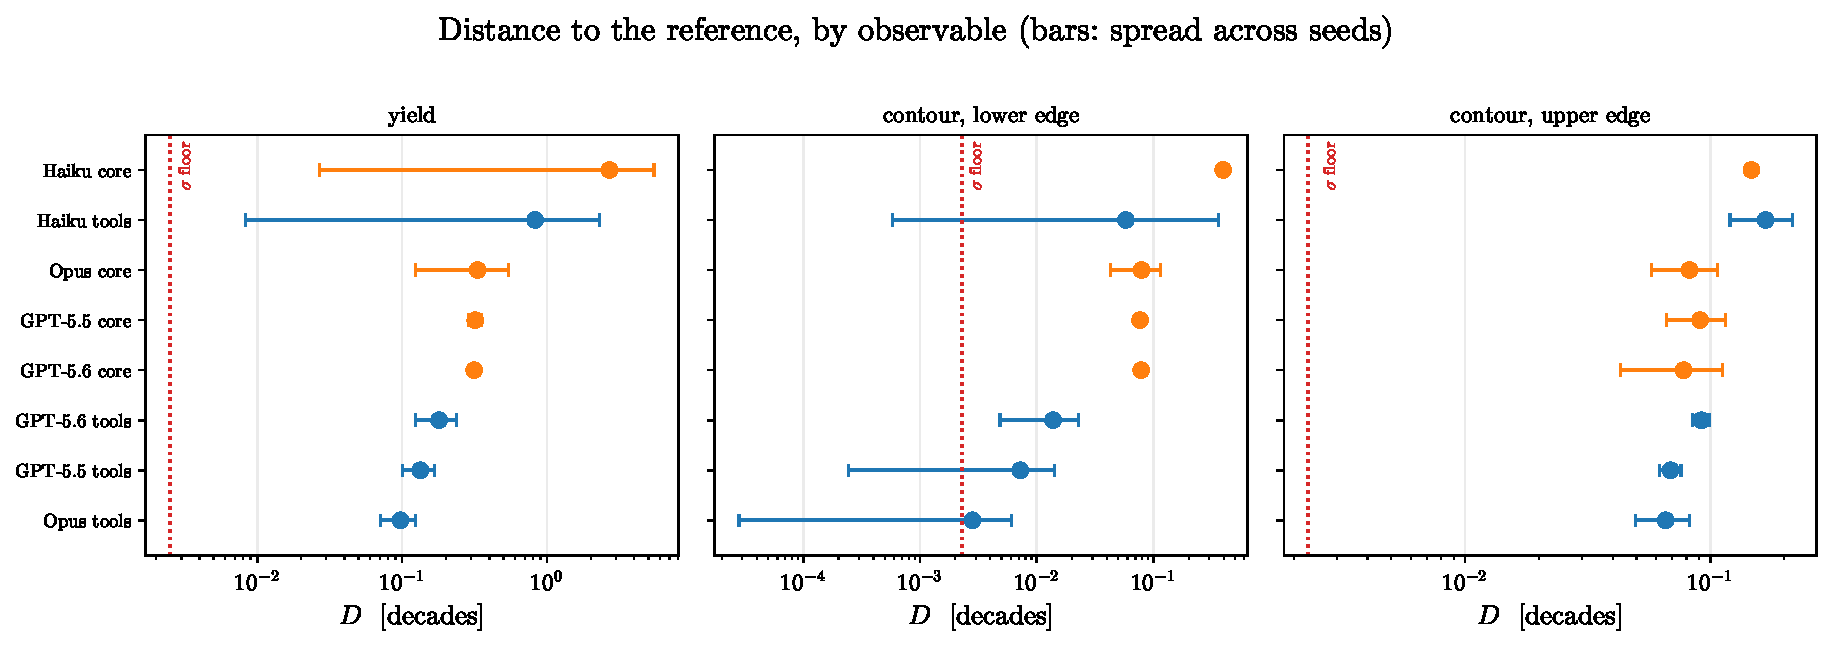
\includegraphics[width=\textwidth]{figures/campaign_summary.pdf}
  \caption{Distance to the reference for each observable. Bars are the spread
  across seeds; the dotted line is the measured $\sigma$ floor. Note the
  logarithmic axis and that the ordering is \emph{not} preserved between panels.}
  \label{fig:campaign}
\end{figure}

\subsection{What the numbers say}

\paragraph{Tools help, by a factor of two to three on yields.} Median $D$ falls
from $\simeq0.32$ dex (core) to $0.10$--$0.18$ dex (tooled) for the three
capable systems. In score terms that is $0.47$--$0.49$ against $0.66$--$0.80$.
The core arms are typically off by a factor of two; the tooled arms by
$25$--$50\%$.

\paragraph{The tool's benefit is concentrated on one edge.} This is the result
that pooling would have hidden:

\begin{center}
\begin{tabular}{lcc}
\toprule
system & lower edge, core $\to$ tools & upper edge, core $\to$ tools \\ \midrule
Opus 4.8      & $0.0791\to0.0028$ \quad($28\times$) & $0.0823\to0.0658$ \quad($1.25\times$) \\
Codex GPT-5.5 & $0.0767\to0.0072$ \quad($11\times$) & $0.0909\to0.0689$ \quad($1.32\times$) \\
Codex GPT-5.6 & $0.0784\to0.0138$ \quad($5.7\times$) & $0.0778\to0.0921$ \quad($0.84\times$) \\
\bottomrule
\end{tabular}
\end{center}

The tool buys between $6\times$ and $28\times$ on the lower edge and
\emph{nothing} on the upper edge, where both arms sit at $0.07$--$0.09$ dex.
This is not an agent failure: the upper edge is set by parents decaying just
below the production cut, a region that every naive decay-length sampling
scheme --- the served tool, hand-written agent code, and the pre-2026-08-07
reference alike --- under-resolves in the same way. It is a shared
methodological blind spot, and as a grading stage it currently discriminates
nothing.

\paragraph{The two arms fail differently.} Figure~\ref{fig:diagnostics}(a):
tooled cells' yield error grows by $\simeq3.5\times$ from the weakest to the
strongest declared coupling, the signature of a lifetime-resolution problem;
core cells are flat at $\simeq0.32$ dex at every coupling, the signature of an
overall normalisation offset. Same $D$ ordering, different diseases.

\begin{figure}[htbp]\centering
  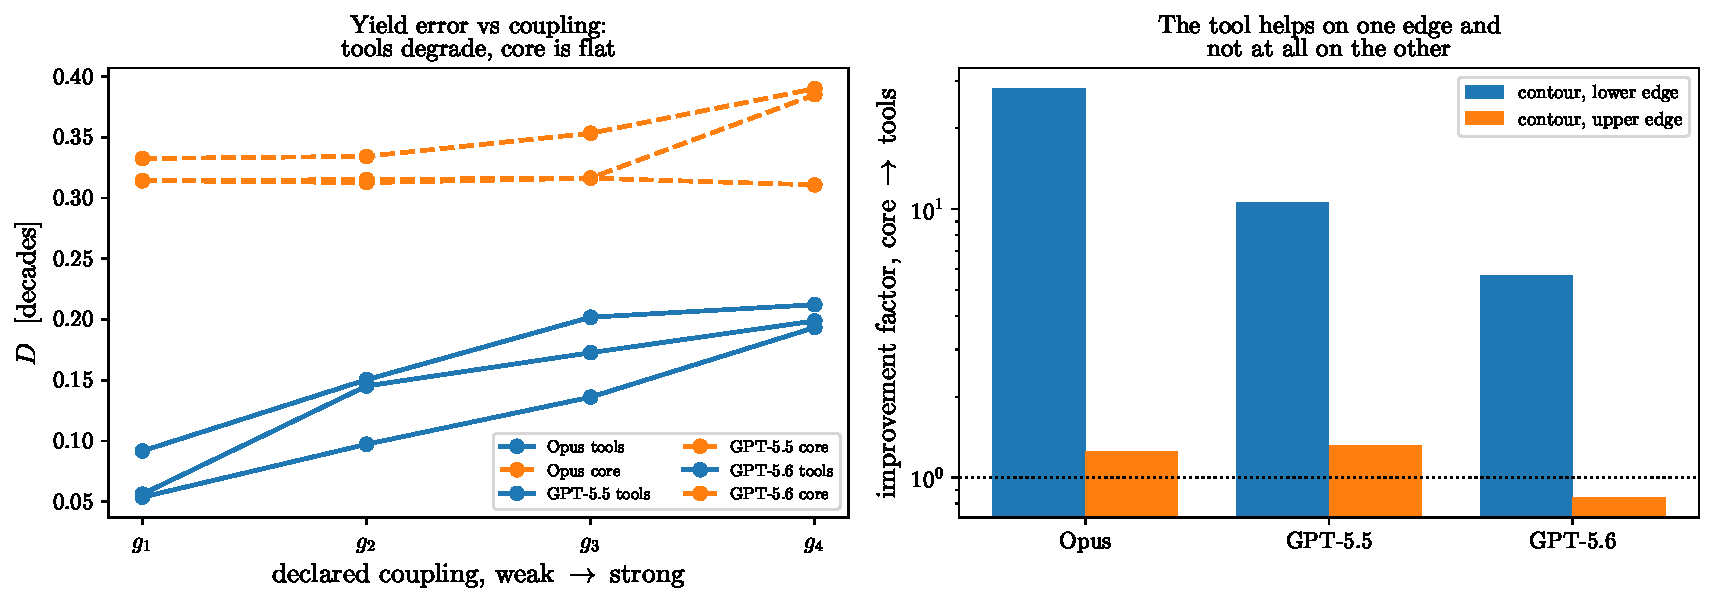
\includegraphics[width=\textwidth]{figures/diagnostics.pdf}
  \caption{(a) Yield error against declared coupling. (b) Improvement factor
  from core to tools, by contour edge.}
  \label{fig:diagnostics}
\end{figure}

\paragraph{Capability and reliability are separate axes.} Codex GPT-5.6 core has
a slightly better median than Opus core ($0.314$ vs $0.332$) while being roughly
twenty times more reproducible (sd $0.011$ vs $0.208$). Haiku's rows carry sd
larger than $D$ and should be read as unstable rather than as a central value.

% auto-generated by hepbench-analysis lib/make_metric_figures.py -- do not edit
\begin{table}[htbp]\centering\small
\begin{tabular}{llrrrrrr}\toprule
system & arm & $D$ & IQR & sd & $n$ & $z$ & $10^{-D}$\\\midrule
Haiku 4.5 & tools & 0.8265 & [0.2443, 1.9721] & 1.4743 & 5 & 331.3 & 0.149\\
Haiku 4.5 & core & 2.6947 & [1.0014, 4.2619] & 2.7747 & 4 & 1080.1 & 0.002\\
Opus 4.8 & tools & 0.0975 & [0.0502, 0.3251] & 0.0269 & 5 & 39.1 & 0.799\\
Opus 4.8 & core & 0.3320 & [0.3077, 0.4701] & 0.2081 & 5 & 133.1 & 0.466\\
Codex GPT-5.5 & tools & 0.1336 & [0.0584, 0.2522] & 0.0333 & 5 & 53.5 & 0.735\\
Codex GPT-5.5 & core & 0.3195 & [0.3055, 0.3680] & 0.0314 & 5 & 128.1 & 0.479\\
Codex GPT-5.6 & tools & 0.1797 & [0.0547, 0.5222] & 0.0559 & 5 & 72.0 & 0.661\\
Codex GPT-5.6 & core & 0.3138 & [0.3052, 0.3575] & 0.0114 & 5 & 125.8 & 0.486\\
Opus 4.8 & bare v1 & 0.2944 & [0.2862, 0.3242] & -- & 1 & 118.0 & 0.508\\
Opus 4.8 & bare v2 & 0.5732 & [0.3595, 0.8456] & -- & 1 & 229.7 & 0.267\\
\bottomrule\end{tabular}
\caption{Yield accuracy at the 48 declared points.}\label{tab:yield}
\end{table}
\begin{table}[htbp]\centering\small
\begin{tabular}{llrrrrrr}\toprule
system & arm & $D$ & IQR & sd & $n$ & $z$ & $10^{-D}$\\\midrule
Haiku 4.5 & tools & 0.0580 & [0.0377, 0.5858] & 0.3033 & 3 & 25.3 & 0.875\\
Haiku 4.5 & core & 0.3955 & -- & -- & 1 & 172.6 & 0.402\\
Opus 4.8 & tools & 0.0028 & [0.0022, 0.0087] & 0.0032 & 5 & 1.2 & 0.994\\
Opus 4.8 & core & 0.0791 & [0.0728, 0.1382] & 0.0361 & 5 & 34.5 & 0.833\\
Codex GPT-5.5 & tools & 0.0072 & [0.0034, 0.0166] & 0.0070 & 5 & 3.2 & 0.984\\
Codex GPT-5.5 & core & 0.0767 & [0.0730, 0.0847] & 0.0045 & 5 & 33.5 & 0.838\\
Codex GPT-5.6 & tools & 0.0138 & [0.0067, 0.0234] & 0.0090 & 5 & 6.0 & 0.969\\
Codex GPT-5.6 & core & 0.0784 & [0.0761, 0.0796] & 0.0017 & 5 & 34.2 & 0.835\\
Opus 4.8 & bare v1 & 0.0691 & [0.0654, 0.0877] & -- & 1 & 30.1 & 0.853\\
Opus 4.8 & bare v2 & 0.2443 & [0.2335, 0.2625] & -- & 1 & 106.6 & 0.570\\
\bottomrule\end{tabular}
\caption{Reach contour, lower (weak-coupling) edge.}\label{tab:lo}
\end{table}
\begin{table}[htbp]\centering\small
\begin{tabular}{llrrrrrr}\toprule
system & arm & $D$ & IQR & sd & $n$ & $z$ & $10^{-D}$\\\midrule
Haiku 4.5 & tools & 0.1682 & [0.1194, 0.2602] & 0.0479 & 3 & 73.4 & 0.679\\
Haiku 4.5 & core & 0.1471 & -- & -- & 1 & 64.2 & 0.713\\
Opus 4.8 & tools & 0.0658 & [0.0625, 0.0967] & 0.0162 & 5 & 28.7 & 0.859\\
Opus 4.8 & core & 0.0823 & [0.0391, 0.0968] & 0.0246 & 5 & 35.9 & 0.827\\
Codex GPT-5.5 & tools & 0.0689 & [0.0582, 0.0891] & 0.0070 & 5 & 30.1 & 0.853\\
Codex GPT-5.5 & core & 0.0909 & [0.0709, 0.0970] & 0.0243 & 5 & 39.7 & 0.811\\
Codex GPT-5.6 & tools & 0.0921 & [0.0749, 0.1087] & 0.0075 & 5 & 40.2 & 0.809\\
Codex GPT-5.6 & core & 0.0778 & [0.0222, 0.0940] & 0.0347 & 5 & 34.0 & 0.836\\
Opus 4.8 & bare v1 & 0.0515 & [0.0461, 0.0839] & -- & 1 & 22.5 & 0.888\\
Opus 4.8 & bare v2 & 0.1143 & [0.0699, 0.2112] & -- & 1 & 49.9 & 0.769\\
\bottomrule\end{tabular}
\caption{Reach contour, upper (strong-coupling) edge.}\label{tab:hi}
\end{table}


\section{Rejected alternatives}\label{sec:rejected}

\paragraph{$\exp(-z^2/2)$ with $z=D/\sigma_{\mathrm{ref}}$.} The previous
proposal. With the rebuilt reference it awards every cell in the campaign
exactly $0.000$, and it gets worse each time the reference improves. A better
reference must not compress all models to zero.

\paragraph{$\sigma_{\mathrm{tot}}=\sigma_{\mathrm{ref}}\oplus\sigma_{\mathrm{agent\;spread}}$.}
Standardising by the agents' own trial-to-trial spread makes the scale depend on
how erratic the agents are, so sloppier fleets are graded more leniently. It is
circular and was rejected.

\paragraph{A chosen accuracy scale, e.g.\ $1/(1+(D/0.2)^2)$.} Workable and
well-behaved, but it puts an arbitrary constant at the centre of every published
score. $10^{-D}$ achieves the same discrimination with nothing to defend.

\paragraph{Comparison against \texttt{\_per\_mass.peak}.} The reference's peak is
the maximum of its internal 400-point scan, at a coupling the declared set never
samples; comparing it to the maximum of an agent's own grid measures the grid
mismatch. It reported $\simeq0.48$ dex for cells whose band edges agreed to
$0.005$--$0.03$ dex.

\paragraph{The band ladder.} \texttt{band\_coarse/mid/fine} scored one
measurement at three hand-chosen thresholds for $40\%$ of the rubric weight.

\section{Caveats}\label{sec:caveats}

\begin{enumerate}
\item Per-point $\sigma$ is not implemented; $z$ is indicative
  (\S\ref{sec:z}). $D$, IQR and $10^{-D}$ are unaffected.
\item Sample sizes are recoverable and provenance-checkable for the
  \emph{tooled} arm only. The core arms emit no tool output, so nothing can be
  tied to the graded scan: of twenty core trials, ten leave an agent-invented
  metadata file, four leave only binary arrays, and six leave nothing. The
  tools-versus-core comparison cannot be made on that axis. The asymmetry is
  itself a result.
\item Agents are not asked to report their own uncertainties. Requiring it would
  permit a proper pull or $\chi^2$ and would improve the benchmark on its own
  terms, since quoting an uncertainty is part of doing the calculation.
\item The upper contour edge currently measures a limitation shared by every
  arm and by the reference's own former implementation. Until the served tool's
  decay-length sampling is corrected, that stage should be reported but not
  weighted as a discriminator.
\item The served tools and the reference share an implementation lineage. This
  is harmless for exact quantities and for converged approximations, but it
  means the benchmark cannot detect an error the two share --- which is
  precisely what happened before 2026-08-07. The defence is convergence testing
  of every discretisation parameter, not separate implementations.
\end{enumerate}

\vspace{1em}
\noindent\rule{\textwidth}{0.4pt}\\[0.3em]
{\small Figures and tables are generated by
\texttt{lib/make\_metric\_figures.py} in \texttt{hepbench-analysis} directly from the preserved
campaign trials. The reference rebuild is documented in
\texttt{benchmarks/llp_forward/soln/notes/strata\_convergence.md} and
\texttt{benchmarks/llp\_forward/soln/reference/strata\_fix.ipynb}.}

\end{document}
